\documentclass[
	% -- opções da classe memoir --
	12pt,				% tamanho da fonte
	%openright,			% capítulos começam em pág ímpar (insere página vazia caso preciso)
	oneside,			% para impressão em recto e verso. Oposto a oneside
	a4paper,			% tamanho do papel. 
	% -- opções da classe abntex2 --
	%chapter=TITLE,		% títulos de capítulos convertidos em letras maiúsculas
	%section=TITLE,		% títulos de seções convertidos em letras maiúsculas
	%subsection=TITLE,	% títulos de subseções convertidos em letras maiúsculas
	%subsubsection=TITLE,% títulos de subsubseções convertidos em letras maiúsculas
	% -- opções do pacote babel --
	english,			% idioma adicional para hifenização
	french,				% idioma adicional para hifenização
	spanish,			% idioma adicional para hifenização
	brazil,				% o último idioma é o principal do documento
	]{abntex2}


% ---
% PACOTES
% ---

% ---
% Pacotes fundamentais 
% ---
\usepackage{pslatex}			% Usa a fonte Latin Modern
\usepackage[T1]{fontenc}		% Selecao de codigos de fonte.
\usepackage[utf8]{inputenc}		% Codificacao do documento (conversão automática dos acentos)
\usepackage{indentfirst}		% Indenta o primeiro parágrafo de cada seção.
\usepackage{color}				% Controle das cores
\usepackage{graphicx}			% Inclusão de gráficos
\usepackage{microtype} 			% para melhorias de justificação
\usepackage{transparent}
\usepackage{eso-pic}
\usepackage{float}
\usepackage{array}
\usepackage{epstopdf}
\usepackage{url}
% ---

% ---
% Pacotes adicionais, usados no anexo do modelo de folha de identificação
% ---
\usepackage{multicol}
\usepackage{multirow}
% ---
	
% ---
% Pacotes adicionais, usados apenas no âmbito do Modelo Canônico do abnteX2
% ---
%\usepackage{lipsum}				% para geração de dummy text
% ---

% ---
% Pacotes de citações
% ---
%\usepackage[brazilian,hyperpageref]{backref}	 % Paginas com as citações na bibl
%\usepackage[alf]{abntex2cite}	% Citações padrão ABNT

% --- 
% CONFIGURAÇÕES DE PACOTES
% --- 

% ---
% Configurações do pacote backref
% Usado sem a opção hyperpageref de backref
%\renewcommand{\backrefpagesname}{Citado na(s) página(s):~}
% Texto padrão antes do número das páginas
%\renewcommand{\backref}{}
% Define os textos da citação
%\renewcommand*{\backrefalt}[4]{
%	\ifcase #1 %
%		Nenhuma citação no texto.%
%	\or
%		Citado na página #2.%
%	\else
%		Citado #1 vezes nas páginas #2.%
%	\fi}%
% ---

% ---
% Informações de dados para CAPA e FOLHA DE ROSTO
% ---
\titulo{Estatística e Probabilidade\\Trabalho sobre Apresentação de Dados\\Parte 2 - Experimental}
\autor{Profª Drª Mara Lúcia Martins Lopes\\Caio da Silva Pereira\\Gabriel Rodrigues Munhoz\\Heitor Martins da Silva\\Leandro Suzuki Barboza dos Santos\\Rafael Gomes de Oliveira\\Thiago Rissetti Roquetto}
\local{Ilha Solteira, São Paulo}
\data{Setembro de 2017}
\instituicao{%
  Universidade Estadual Paulista  - Unesp
  \par
  Faculdade de Engenharia de Ilha Solteira  - FEIS}
\tipotrabalho{Trabalho científico}
% O preambulo deve conter o tipo do trabalho, o objetivo, 
% o nome da instituição e a área de concentração 
\preambulo{"Estatística é método, ciência e arte."}
% ---

% ---
% Configurações de aparência do PDF final

% alterando o aspecto da cor azul
\definecolor{blue}{RGB}{41,5,195}

% informações do PDF
\makeatletter
\hypersetup{
     	%pagebackref=true,
		pdftitle={\@title}, 
		pdfauthor={\@author},
    	pdfsubject={\imprimirpreambulo},
	    pdfcreator={LaTeX with abnTeX2},
		pdfkeywords={abnt}{latex}{abntex}{abntex2}{relatório técnico}, 
		colorlinks=true,       		% false: boxed links; true: colored links
    	linkcolor=blue,          	% color of internal links
    	citecolor=blue,        		% color of links to bibliography
    	filecolor=magenta,      		% color of file links
		urlcolor=blue,
		bookmarksdepth=4
}
\makeatother
% --- 

% --- 
% Espaçamentos entre linhas e parágrafos 
% --- 

% O tamanho do parágrafo é dado por:
\setlength{\parindent}{1.3cm}

% Controle do espaçamento entre um parágrafo e outro:
\setlength{\parskip}{0.2cm}  % tente também \onelineskip

% ---
% compila o indice
% ---
\makeindex
% ---
\usepackage{fancyhdr}
\fancyhead{}
\fancyfoot{}
\lhead{Trabalho sobre Ajustagem Mecânica}
\rhead{\thepage}

\AddToShipoutPicture{

\put(0,0){

\parbox[b][\paperheight]{\paperwidth}{%

\vfill

\centering

{\transparent{0.1}\includegraphics[scale=2]{../../../Imagens/SA03x.jpg}  }%

\vfill}}}
% ----
% Início do documento
% ----
\begin{document}

\begin{minipage}[c][1.5cm][c]{3cm} % a primeira minipágina tem uma altura de 1.5cm e uma largura de 3cm.

\includegraphics[scale=0.6]{../../../Imagens/barraunesp-assvisual.png} 

\end{minipage}

% Seleciona o idioma do documento (conforme pacotes do babel)
%\selectlanguage{english}
\selectlanguage{brazil}

% Retira espaço extra obsoleto entre as frases.
\frenchspacing 

% ----------------------------------------------------------
% ELEMENTOS PRÉ-TEXTUAIS
% ----------------------------------------------------------
%\pretextual

% ---
% Capa
% ---
\imprimircapa
% ---

% ---
% Folha de rosto
% (o * indica que haverá a ficha bibliográfica)
% ---
\imprimirfolhaderosto*

% ---
% inserir o sumario
% ---
\pdfbookmark[0]{\contentsname}{toc}
\tableofcontents*
\newpage

\section[Objetivo]{Objetivo}
\pagestyle{fancy}

A estatística das marcas de carro na cidade de Ilha Solteira.

\newpage
\section[Resumo]{Resumo}

A pesquisa foi realizada com o âmbito de visualizarmos as marcas de carro mais presentes em Ilha Solteira.  O modo como os dados forem coletados evitou que o mesmo carro fosse anotado mais de uma vez e a partir disso montamos uma lista com 86 veículos. A partir desses dados montamos uma tabela de frequência e um gráfico para melhor visualização. O resultado veio ao encontro da teoria, pois, a maior porcentagem foi da marca Volkswagen que é considerada marca de carro popular.  


\newpage
\section[Procedimento Experimental]{Procedimento Experimental}

Após escolhido o tema coletamos os dados nas ruas de Ilha Solteira, anotando a marca dos carros e suas placas para que não houvessem dados repetidos no projeto. Em seguida, realizou-se a análise organizando os dados em uma tabela de distribuição de frequência composta pela frequência absoluta, frequência relativa e a acumulada de ambas.

Por fim, os dados foram transferidos para um gráfico de pizza, para que possamos ter uma melhor visualização das frequências de cada marca. Como os dados coletados são qualitativos nominais apenas apresentamos eles e discutimos, pois, não há forma de calcularmos média, mediana ou moda.


% ---
% inserir lista de ilustrações
% ---
%\pdfbookmark[0]{\listfigurename}{lof}
%\listoffigures*
%\cleardoublepage
% ---

% ---
% inserir lista de tabelas
% ---
%\pdfbookmark[0]{\listtablename}{lot}
%\listoftables*
%\cleardoublepage
% ---

% ---
% inserir lista de abreviaturas e siglas
% ---
%\begin{siglas}
% \item[ABNT] Associação Brasileira de Normas Técnicas
%  \item[abnTeX] ABsurdas Normas para TeX
%\end{siglas}
% ---

% ---
% inserir lista de símbolos
% ---
%\begin{simbolos}
  %\item[$ \Gamma $] Letra grega Gama
  %\item[$ \Lambda $] Lambda
  %\item[$ \zeta $] Letra grega minúscula zeta
  %\item[$ \in $] Pertence
%\end{simbolos}
% ---

% ----------------------------------------------------------
% ELEMENTOS TEXTUAIS
% ----------------------------------------------------------
\newpage

\section[Resultados e Discussão]{Resultados e Discussão}
\pagestyle{fancy}

Os dados brutos obtidos foram:

\begin{center}
\begin{table}[H]
\begin{center}
\begin{tabular}{llllllllll}


Chevrolet & Fiat & Ford & Honda & Hyundai & Kia & Mitsubishi & Toyota & Volkswagen & Renault \\ 

Chevrolet & Fiat & Ford & Honda & Hyundai &  &  & Toyota & Volkswagen &  \\

Chevrolet & Fiat & Ford &  & Hyundai &  &  & Toyota & Volkswagen &  \\ 

Chevrolet & Fiat & Ford &  & Hyundai &  &  & Toyota & Volkswagen &  \\

Chevrolet & Fiat & Ford &  & Hyundai &  &  & Toyota & Volkswagen &  \\ 

Chevrolet & Fiat & Ford &  & Hyundai &  &  & Toyota & Volkswagen &  \\

Chevrolet & Fiat & Ford &  & Hyundai &  &  & Toyota & Volkswagen &  \\ 

Chevrolet & Fiat & Ford &  & Hyundai &  &  &  & Volkswagen &  \\

Chevrolet & Fiat & Ford &  & Hyundai &  &  &  & Volkswagen &  \\ 

Chevrolet & Fiat & Ford &  &  &  &  &  & Volkswagen &  \\

Chevrolet & Fiat & Ford &  &  &  &  &  & Volkswagen &  \\ 

Chevrolet & Fiat &  &  &  &  &  &  & Volkswagen &  \\

Chevrolet & Fiat &  &  &  &  &  &  & Volkswagen &  \\ 

Chevrolet &  &  &  &  &  &  &  & Volkswagen &  \\

Chevrolet &  &  &  &  &  &  &  & Volkswagen &  \\ 

Chevrolet &  &  &  &  &  &  &  & Volkswagen &  \\

Chevrolet &  &  &  &  &  &  &  & Volkswagen &  \\ 

Chevrolet &  &  &  &  &  &  &  & Volkswagen &  \\

Chevrolet &  &  &  &  &  &  &  & Volkswagen &  \\ 

 &  &  &  &  &  &  &  & Volkswagen &  \\

 &  &  &  &  &  &  &  & Volkswagen &  \\ 

 &  &  &  &  &  &  &  & Volkswagen & \\

\end{tabular}
\end{center}

\end{table}
\end{center}

Tais dados foram organizados em uma tabela de distribuição de frequência:

\begin{center}
\begin{table}[H]
\caption{Distribuição de frequência do número de carros por marca em Ilha Solteira}
\begin{center}
\begin{tabular}{>{\centering\arraybackslash}m{2cm}|>{\centering\arraybackslash}m{2cm}|>{\centering\arraybackslash}m{2cm}|>{\centering\arraybackslash}m{2cm}|>{\centering\arraybackslash}m{2cm}}

\hline
Marca & Frequência Absoluta & Frequência Relativa$(\%)$ & Frequência Absoluta Acumulada & Frequência Relativa Acumulada \\ 
\hline
Chevrolet & 19 & 22,09 & 19 & 22,09 \\
\hline
Fiat & 13 & 15,11 & 32 & 37,20 \\
\hline
Ford & 11 & 12,79 & 43 & 49,99 \\
\hline
Honda & 2 & 2,36 & 45 & 52,35 \\
\hline
Hyundai & 9 & 10,46 & 54 & 62,81 \\
\hline
Kia & 1 & 1,16 & 55 & 63,97 \\
\hline
Mitsubishi & 1 & 1,16 & 56 & 65,13 \\
\hline
Toyota & 7 & 8,14 & 63 & 73,27 \\
\hline
Volkswagen & 22 & 25,57 & 85 & 98,84 \\
\hline
Renault & 1 & 1,16 & 86 & 100,00 \\
\hline
Total & 86 & 100,00 & -- & -- \\

\end{tabular}
\end{center}
\legend{Fonte: Elaborado pelo Autor}
\end{table}
\end{center}

E por fim, foi criado um gráfico de pizza para uma melhor visualização dessa distribuição de marcas de carro na cidade de Ilha Solteira:

\begin{figure}[H]
\begin{center}
\caption{Gráfico de Pizza do número de carros por marca em Ilha Solteira}

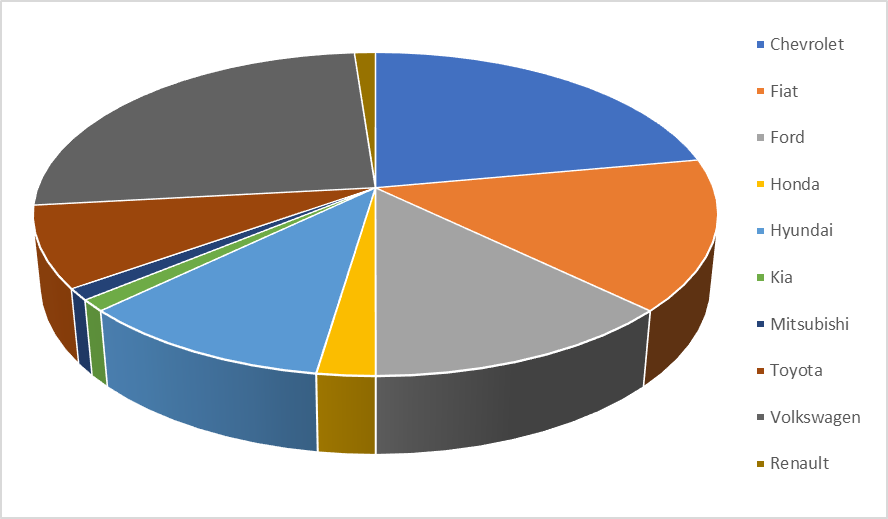
\includegraphics[scale=0.8]{grafico8.jpg}  

\legend{Fonte: Elaborado pelo Autor}
\end{center}
\end{figure}

E por meio de uma análise dos dados verificamos que a marca Volkswagen possui uma maior frequência na cidade de Ilha Solteira $(25\%)$, enquanto outras marcas como Kia, Mitsubishi, Renault e até mesmo a Honda não possuem uma presença tão grande $(<3\%$ cada$)$. 

Podemos agregar tal resultado ao fato de não existirem concessiorárias dessas 4 últimas marcas tão presentes no interior paulista e ao valor dos carros, pois, a marca Volkswagen possui mais veículos de baixo custo do que as outras. O resultado foi ao encontro do que esperávamos, pois, a marca mais presente na cidade é também considerada uma marca de carros populares e por causa disso possui mais exemplares na rua.

\newpage
\section[Conclusão]{Conclusão}
\pagestyle{fancy}

A análise feita da estatística das marcas de carro na cidade de Ilha Solteira, gerou resultados importantes que são muitas vezes utilizados em pesquisas de mercados para certos estabelecimentos. 

As marcas que mais se destacaram foram as que possuem carros populares, assim dizendo, carros com um valor mais acessível para a população. Já as marcas com carros um pouco mais caros se mostraram pouco presentes, ainda mais por não possuírem pontos de venda tão próximos de Ilha Solteira. 

Portanto, os dados coletados foram de extrema importância e refletiram de um modo geral como as marcas de carro estão distribuídas na cidade de Ilha Solteira.  


% ----------------------------------------------------------
% Glossário
% ----------------------------------------------------------
%
% Consulte o manual da classe abntex2 para orientações sobre o glossário.
%
%\glossary


\end{document}